\section{Universidad de Chile}

\subsection{Breve consideración histórica de la institución con referencia a su misión}
\label{historia}

La Universidad de Chile es una institución de educación superior de carácter nacional y pública,
que asume con compromiso y vocación de excelencia la formación de personas y la contribución
al desarrollo espiritual y material de la Nación. Construyendo liderazgo en el desarrollo innovador
de las ciencias y las tecnologías, las humanidades y las artes, a través de sus funciones de docencia,
creación y extensión, con especial énfasis en la investigación y el postgrado. Promueve el ejercicio
de una ciudadanía preparada, crítica, con conciencia social y responsabilidad ética, de acuerdo a los
valores de tolerancia, pluralismo y equidad, independencia intelectual y libertad de pensamiento.
Así como también del respeto, promoción y preservación de la diversidad en todos los ámbitos de
su quehacer.

\begin{figure}[ht!]
\centering
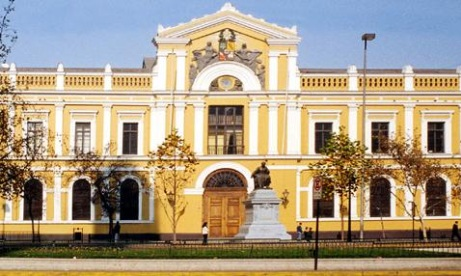
\includegraphics[width=\columnwidth]{./pictures/uchile.jpg}
\caption{Casa central de la Universidad de Chile}
\end{figure}

Es la más antigua del país (data de 1842) y una de las de mayor prestigio y tradición de América
Latina, como lo prueban múltiples reconocimientos nacionales e internacionales. En el plano
nacional, la Universidad de Chile recibe en términos relativos el mayor número de estudiantes con
los mejores puntajes de ingreso al sistema de educación superior, cuenta con un cuerpo académico
de excelencia, con una alta productividad en el campo científico y de la creación artística y cultural,
y está permanentemente vinculada a la reflexión y solución de los problemas nacionales.

Desde una perspectiva de regulación externa de la calidad, la Universidad participó en la
primera experiencia voluntaria de acreditación institucional en Chile (año 2004), habiendo sido
acreditada por la Comisión Nacional de Acreditación de Pregrado, (CNAP), en todas las áreas
consideradas (gestión estratégica, docencia de pregrado, investigación y creación, docencia de
postgrado, vinculación con el medio e infraestructura) y por el máximo período considerado
para estos efectos por el organismo citado (siete años). Durante el año 2011 la Universidad
se sometió a un segundo proceso de acreditación ante la Comisión Nacional de Acreditación
(CNA), manteniendo los siete años en todas las áreas consideradas. En lo internacional, mantiene
activas relaciones de intercambio científico, pedagógico, cultural y artístico con destacadas
universidades del continente americano, Europa y otros continentes y ocupa una alta posición
a nivel latinoamericano en rankings universitarios tales como el del Jiao Tong Institute de la
Universidad de Shanghai, y el del SCImago Research Group, de España.

Los orígenes de la Universidad de Chile se encuentran en las primeras universidades
conventuales que se fundan en el país durante el siglo XVII, en el período colonial, y que reciben
autorización real y pontificia para otorgar títulos de bachiller, licenciado, maestro y doctor en
filosofía y teología. Más tarde, en 1738, se crea una universidad real, docente y de claustro,
a la que se llama de San Felipe, en honor del rey Felipe V, con Facultades de leyes, teología,
medicina y matemáticas. Con motivo de la independencia del imperio español, esta institución
se adapta progresivamente a las nuevas circunstancias de la vida republicana y pasa a llamarse
Universidad del Estado de Chile, luego de la República de Chile, y finalmente, Universidad de
Chile. En 1842 se dicta una ley orgánica de acuerdo a la cual la Universidad de Chile recibe la
función de superintendencia de todos los niveles de la enseñanza del país. Asimismo, se le encarga
propagar la afición por los estudios superiores, promover la investigación y la divulgación científica
y literaria y servir de auxiliar a los trabajos de las diversas dependencias de la administración del
Estado. Cinco Facultades académicas forman entonces la universidad: Humanidades y Filosofía,
Ciencias Matemáticas y Físicas, Leyes y Ciencias Políticas, Medicina, y Teología. Estas Facultades
tenían una función eminentemente científica, puesto que la labor docente de la Universidad quedaba
radicada en el Instituto Nacional, fundado en 1811 e inaugurado el 10 de agosto de 1813. 
El 9 de enero de 1879 se dictó un nuevo estatuto
que transformó a la Universidad en una institución de finalidad docente.

En 1931 se dicta una nueva ley orgánica que consagra la doble función científica y docente de
la Universidad. A partir de entonces, y durante treinta años, se mantiene un crecimiento sostenido
de la Corporación. Crece el número de sus facultades e institutos, de sus centros de investigación
y de sus carreras y programas académicos. Las actividades de extensión reciben también un fuerte
impulso, creándose la Orquesta Sinfónica de Chile y el Teatro Experimental de la Universidad, en
1941; el Museo de Arte Popular Americano, en 1943; el Coro Universitario y el Ballet Nacional,
en 1945; y el Museo de Arte Contemporáneo, en 1947. Asimismo, se inicia la radiotelefonía
universitaria, y se realizan las Escuelas Internacionales de Temporada, que atraen a profesores y
estudiantes de todo el continente y llevan los contenidos de la ciencia y la cultura al gran público.
La realización de escuelas de temporada en provincia es el primer paso para la fundación de los
centros universitarios regionales, que luego se convierten en las distintas sedes que llega a tener
la Universidad en las principales ciudades del país. De estas sedes derivarán, más tarde, diversas
universidades autónomas.

Junto con formar profesionales y graduados, la Universidad de Chile ha cumplido a lo largo
de su historia una labor de primera importancia a nivel nacional, a la vez que se ha constituido en
uno de los principales centros de creación científica y artística y de irradiación cultural de América
Latina. La primera de las grandes tareas que emprende fue la organización de un sistema nacional
de educación, en el siglo XIX. En el siglo XX contribuye decisivamente a ampliar a todo el país
la cobertura de la atención primaria en salud, a superar el problema de la desnutrición infantil,
a la construcción de grandes obras de infraestructura productiva y energética, al estudio de los
materiales de construcción y al desarrollo de la ingeniería sismorresistente, con lo que se aminoran
en gran medida los efectos de los terremotos, y al desarrollo productivo exportador, especialmente
en las áreas silvoagropecuarias y minera, entre otras grandes tareas. En lo internacional, es
reconocida su acción en prácticamente todas las áreas.

En la actualidad, y para desarrollar sus actividades, la Universidad de Chile se organiza en
14 facultades, 4 institutos interdisciplinarios y tres centros. Las Facultades son: Arquitectura y
Urbanismo; Artes; Ciencias; Ciencias Agronómicas; Ciencias Físicas y Matemáticas; Ciencias
Forestales y Conservación de la Naturaleza; Ciencias Químicas y Farmacéuticas; Ciencias Sociales;
Ciencias Veterinarias y Pecuarias; Derecho; Economía y Negocios; Filosofía y Humanidades;
Medicina; y Odontología. Los Institutos son: Instituto de Asuntos Públicos (INAP); Instituto
de Estudios Internacionales (IEI); Instituto de Nutrición y Tecnología de los Alimentos (INTA)
e Instituto de Comunicación e Imagen (ICEI). Deben destacarse también el Hospital Clínico
José Joaquín Aguirre, el Liceo Experimental Manuel de Salas, una gran institucionalidad cultural
(Orquesta Sinfónica, Ballet Nacional, Coro de la Universidad de Chile, Teatro Nacional, Museo de
Arte Contemporáneo, Museo de Arte Popular Americano, Archivo Andrés Bello y otros), la Radio
de la Universidad de Chile y muchas otras instancias que se encuentran adscritas a Facultades e
Institutos.

La Universidad de Chile cuenta con una matrícula superior a 31 mil estudiantes de pregrado
distribuidos en 69 programas de estudio, los cuales incluyen 55 carreras profesionales y 
14 licenciaturas terminales. Además ofrece más de un centenar de programas de especialización en
diversas áreas.

En el período comprendido entre los años 2002 y 2017 la oferta de vacantes regulares (vía
PSU) ha aumentado desde los 4.000 a los 5.453 cupos anuales, y la oferta global de vacantes ha
crecido por sobre los 6.309 cupos anuales (para todas las vías de ingreso). En el año 2017, para un
total de 5.453 vacantes regulares, se registró un total de 17.910 postulaciones a la Universidad de
Chile.

% En el año <#ano_estadistica_matricula#>, el <.#porcentaje_matriculados_UCH#.>\% de los estudiantes que alcanzaron puntajes nacionales se matricularon
% en la Universidad de Chile; de igual forma, de entre todos los puntajes nacionales, el <.#porcentaje_colegio_municipal#.>\% de los
% provenientes de colegios municipales y el <.#porcentaje_colegio_subvencionados#.>\% de los provenientes de colegios subvencionados
% eligieron esta universidad para realizar sus estudios superiores, dando cuenta tanto de la percepción
% positiva que tienen los estudiantes y sus familias de la Universidad de Chile, como de la diversidad
% de éstos y la interacción de la Universidad con el medio social dado su carácter nacional y estatal.

Junto a este énfasis por la excelencia de los alumnos que ingresan, la Universidad de Chile se
esfuerza por fomentar la equidad. Concretamente, ha instituido la Beca de Equidad Universidad de
Chile que cubre la diferencia entre el arancel real y el arancel de referencia y que hasta ahora era
financiada por estos estudiantes a través de un crédito otorgado por el Fondo Solidario de Crédito
Universitario. Considerando que los estudiantes de los dos primeros quintiles de ingreso reciben
del MINEDUC una beca para financiar el arancel de referencia, la Beca de Equidad Universidad
de Chile significa, en los hechos, gratuidad de aranceles para los estudiantes más vulnerables.

% Dado que la Universidad de Chile es la institución de educación superior que matricula la
% mayor cantidad de alumnos dentro de los <.#mejores_puntajes_PSU#.> mejores puntajes en la PSU, es la que obtiene el
% mayor Aporte Fiscal Indirecto (AFI) del sistema educacional chileno.

El sistema de postgrado y postítulo de esta institución es el más grande y complejo del país,
compuesto por 38 programas de doctorado, 116 programas de magíster, 69 programas de título
profesional especialista y 13 cursos de especialización de postítulo, con cerca de 9.290 estudiantes,
todos estos valores vigentes hasta el año 2016.

A nivel de investigación, en el Concurso FONDECYT Regular en el período 2005-2012 la
Universidad de Chile se adjudicó 914 proyectos, lo que corresponde al 26\% del total nacional.
En el año 2012 este concurso adjudicó a la Universidad de Chile fondos por US\$37,8 millones
(\$17.766 millones equivalentes en pesos chilenos). A nivel del Concurso FONDECYT de Iniciación 2012, la
Universidad de Chile se adjudicó 51 de 293 proyectos (17,4\% del total) por un monto de \$3.041
millones, concentrando un 18,8\% del total de fondos asignados a nivel nacional (\$16.196 millones). En
cuanto al Concurso FONDECYT de Postdoctorado 2013, esta casa de estudios se adjudicó 61
de un total de 238 proyectos seleccionados (25,6\% del total) y \$3.779 millones de un total de
\$14.980 millones, correspondiente al 25,2\% del total de recursos asignados en este concurso.

Por otra parte es destacable mencionar que en el período 2010-2016 los académicos de la
Universidad de Chile tuvieron 12.037 publicaciones ISI, la mayor productividad académica a nivel nacional.

En la Universidad de Chile han sido formados la mayor parte de los Presidentes de la
República, incluyendo a Manuel Montt Torres, Federico Errázuriz Zañartu, Domingo Santa María,
Federico Errázuriz Echaurren, Germán Riesco, Pedro Montt, Ramón Barros Luco, Juan Luis
Sanfuentes, Arturo Alessandri Palma, Emiliano Figueroa, Juan Esteban Montero, Pedro Aguirre
Cerda, Gabriel González Videla, Jorge Alessandri Rodríguez, Salvador Allende Gossens, Patricio
Aylwin Azócar, Eduardo Frei Ruiz-Tagle, Ricardo Lagos Escobar y Michelle Bachelet Jeria. La
mayor parte de los ganadores de premios nacionales en las menciones de ciencias, humanidades y
artes son ex-alumnos de esta casa de estudios (180 Premios Nacionales).
%, que representan el <.#porcentaje_premios_UCH_del_total#.>\% del total).
Gabriela Mistral, receptora del Premio Nobel de Literatura (1945), y Pablo Neruda, 
receptor del Premio Nobel de Literatura (1971), fueron miembros de la Universidad de Chile.

Actualmente la Universidad se rige por un nuevo Estatuto que modifica el DFL N$^{\circ}$ 153 de
1981, dando lugar a una nueva institucionalidad: el Rector es la máxima autoridad unipersonal
y representante legal, quien es elegido por los pares académicos por un período de cuatro
años; el Senado Universitario, órgano colegiado con funciones normativas y de lineamientos
estratégicos, compuesto por 36 miembros (27 académicos, 7 estudiantes y 2 representantes del
personal de colaboración) elegidos por sus pares; el Consejo Universitario, órgano colegiado
de carácter ejecutivo, compuesto por el Rector quien lo preside, el Prorrector, los Decanos,
y dos miembros designados por el Presidente de la República; el Consejo de Evaluación, a
cargo de la superintendencia de los procesos de evaluación, calificación y autoevaluación a nivel
institucional e individual, integrado por 5 profesores de la más alta jerarquía académica, quienes
son propuestos por el Rector y nombrados por el Senado Universitario; el Prorrector, quien asesora
al Rector en materias de orden académico, económico-administrativo, jurídico y estudiantil, quien
lo reemplaza en caso de ausencia y coordina la 5 Vicerrectorías: (i) Asuntos Académicos, (ii)
Asuntos Económicos, (iii) Asuntos Estudiantiles y Comunitarios, (iv) Investigación y Desarrollo,
y (v) Extensión y Comunicaciones.

\section{Facultad de Ciencias Físicas y Matemáticas}

\begin{figure}[ht!]
\centering
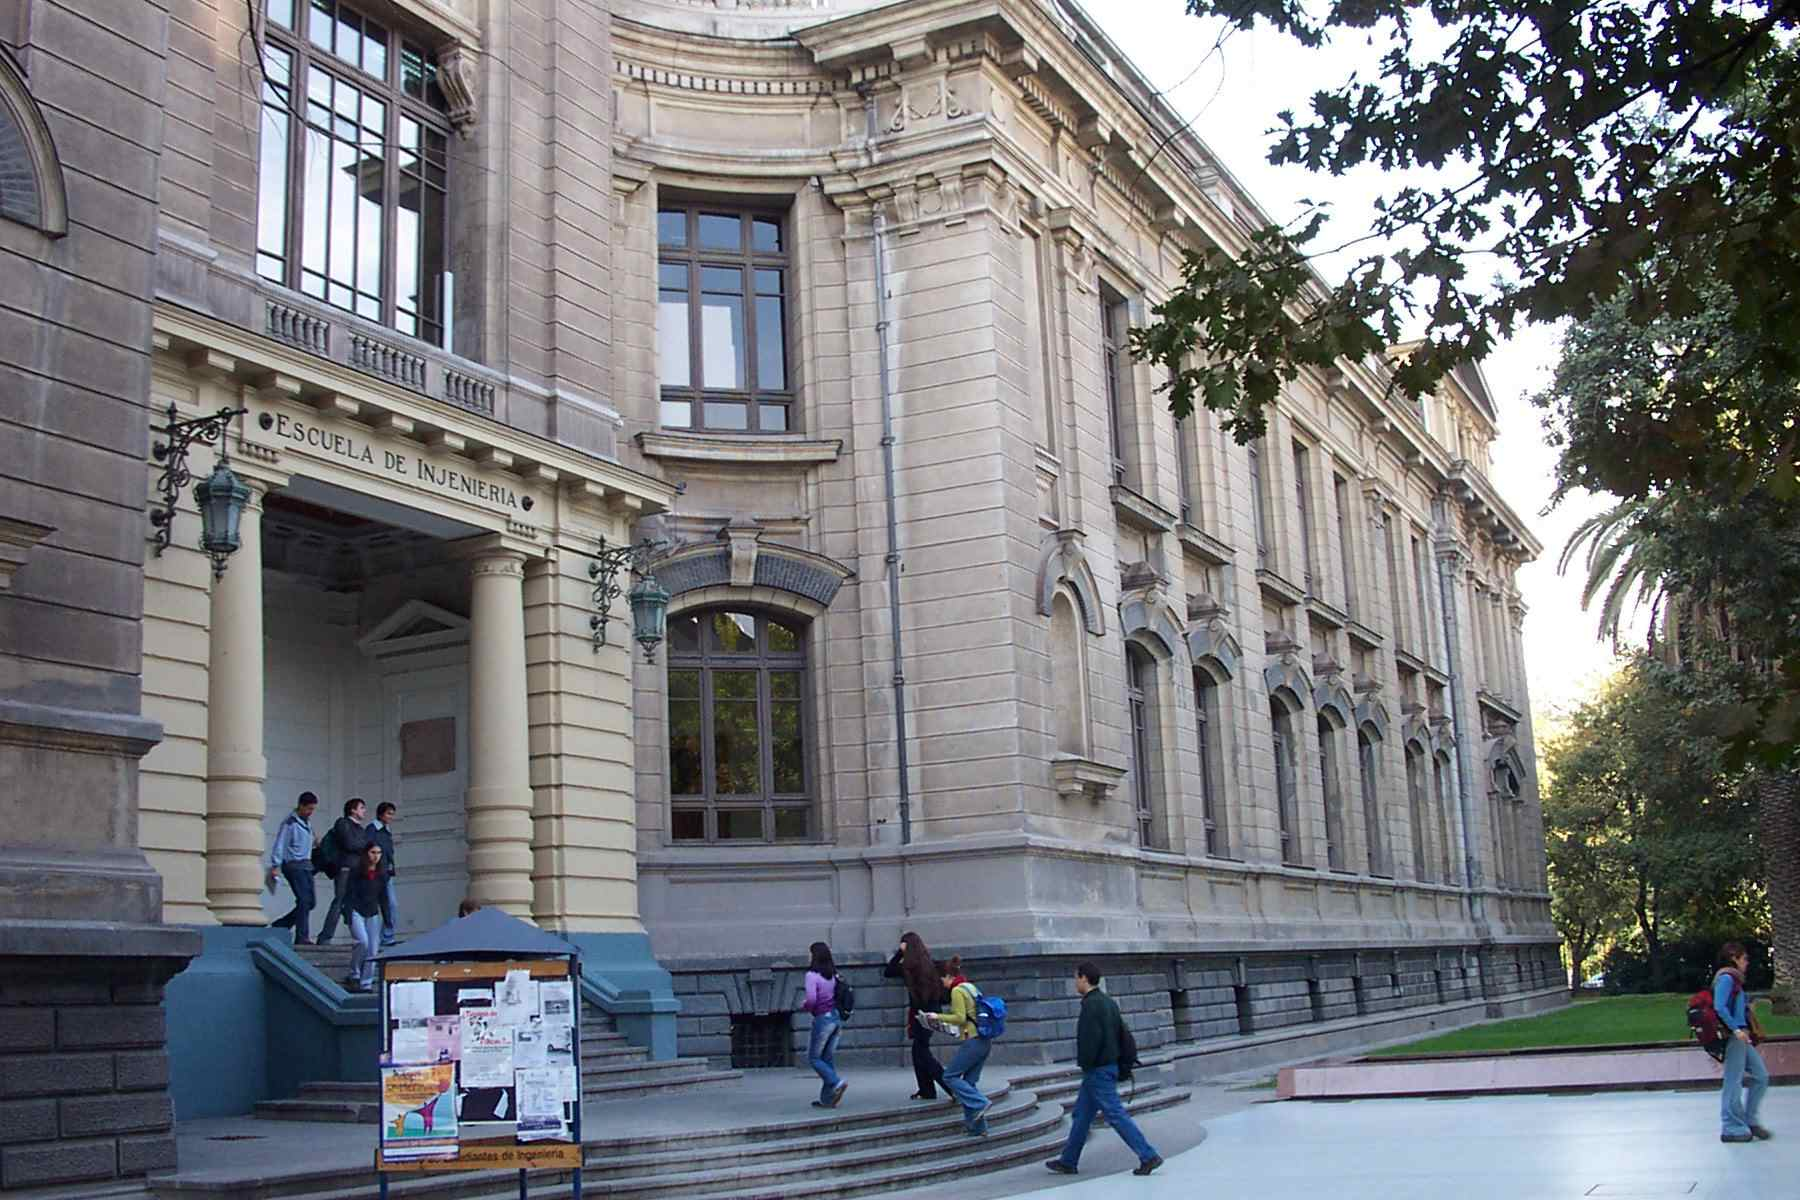
\includegraphics[width=\columnwidth]{./pictures/frontis.jpg}
\caption{Frontis de la entrada principal de la escuela de ingeniería}
\end{figure}

\subsection{Reseña Histórica}

La Facultad de Ciencias Físicas y Matemáticas (FCFM) es tan antigua como la propia Universidad
de Chile, ya que ambas se crearon en el año 1842, bajo el gobierno del Presidente Manuel Bulnes.

En ese entonces, Andrés Bello, quien fuera el primer Rector de la Universidad, le pidió al
ingeniero español, Andrés Antonio Gorbea que dirigiera esta nueva Facultad. Nueve años después,
en 1853, se organizó la enseñanza de la ingeniería propiamente tal impartiendo las especialidades de
Ingeniero Geógrafo, Ingeniero de Minas, Ingeniero de Puentes y Caminos, y también Arquitectura
(carrera que se independizó en 1946).

En 1911 comenzó la construcción de un nuevo edificio para la Facultad, ubicado en Santiago,
en la calle Benavente 850 -actual Beauchef-. La inauguración se realizó el 8 de abril de 1922, ante
la presencia de ministros de Estado, embajadores y el entonces Presidente de la República, Arturo
Alessandri Palma.

Con la creación de la Corporación de Fomento de la Producción (CORFO) en 1939 y de
grandes empresas públicas en los años 40, la Facultad debió adaptar las Escuelas de Ingeniería a la
nueva realidad tecnológica nacional.

Durante la segunda mitad del siglo XX, la FCFM continuó consolidando su liderazgo
en la formación de ingenieros y científicos, contribuyendo al desarrollo del país en áreas
como la electrificación, el agua potable, obras civiles de gran envergadura, el transporte y las
telecomunicaciones.

Como una forma de responder a los desafíos, a partir de los años 60 y hasta la década del 90
se empezaron a crear nuevas carreras como Ingeniería Civil en Matemáticas, en Computación, en
Materiales y, finalmente, en Biotecnología.

Con la llegada del siglo XXI, la Escuela de Ingeniería y Ciencias realizó cambios curriculares
con el objetivo de apoyar la innovación en la enseñanza y el aprendizaje. Para el diseño de estos
cambios, la Facultad adoptó metodologías originadas en el Massachusetts Institute of Technology
(MIT) que fueron incorporadas por las más prestigiosas escuelas de ingeniería del mundo. Dicho
método se conoce como iniciativa CDIO\footnote{Obtenido de \url{http://www.cdio.cl}}, denominada de esta manera para hacer énfasis en las
competencias de concebir, diseñar, implementar y operar sistemas de ingeniería.

En 2011 y como un reflejo de los 170 años de tradición y excelencia, la FCFM comenzó
la construcción del proyecto de infraestructura más importante desarrollado en los últimos 100
años, que se ubica en Beauchef 851, el que se describe en mayor detalle en la Sección \ref{infra_fcfm}
``Infraestructura de la FCFM''.

En la actualidad la Facultad presta importantes servicios de asesoría a organismos, empresas
y corporaciones estatales y privadas en todas las ramas de la ingeniería y la ciencia. Asimismo
continúa innovando y creando soluciones y requerimientos tecnológicos para enfrentar nuevos
escenarios.Dentro de esto, la facultad está trabajando en su nuevo Plan estratégico enmarcado en
el desarrollo del proyecto Ingeniería 2030 [\ref{fcfm_plan_2030}]. En el desarrollo del mismo se han realizado
seminarios, análisis y estudios tendientes a redefinir tanto las carreras como los programas de
postgrado y la articulación entre ellos.

\subsection{Estructura Orgánica de la FCFM}
\label{estruct_org_fcfm}

La estructura Orgánica de la FCFM que se ilustra en la Figura \ref{ograma_fcfm} está compuesta por el Decano,
Vicedecano, Consejo de Facultad, Dirección Académica y de Investigación, Dirección Económica
y Administrativa, División Jurídica, Escuela de Ingeniería y Ciencias, Escuela de Postgrado, 13
Departamentos, y Centros de Investigación y de Servicios. El Reglamento General de Facultades,
Decreto Universitario Exento N$\circ$ 906 de 27 de enero de 2009 [\ref{reg_gen_fac}], describe entre otros puntos
las funciones de las autoridades unipersonales, consejos y departamentos, como se resume a
continuación.

\begin{figure}[ht!]
\centering
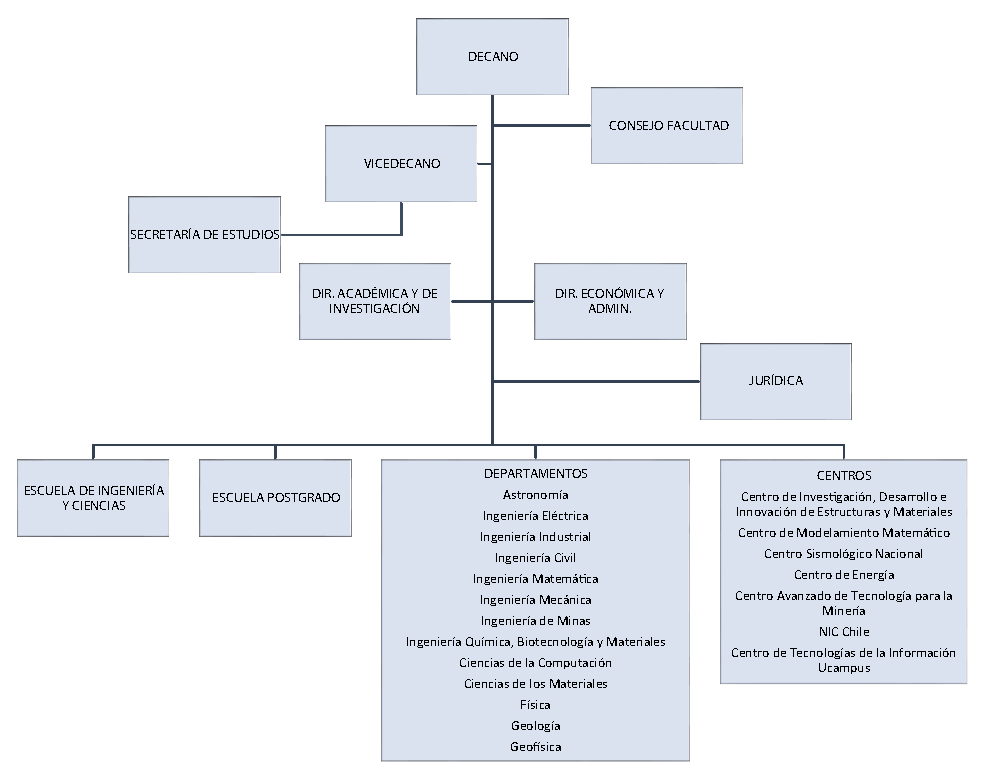
\includegraphics[width=\columnwidth]{./organigramas/organigrama_fcfm.eps}
\caption{Organigrama Facultad de Ciencias Físicas y Matemáticas de la Universidad de Chile}
\label{ograma_fcfm}
\end{figure}

El \textbf{Decano} es la máxima autoridad de la respectiva Facultad y le corresponde la dirección
de ésta, en el contexto de los lineamientos y estrategias emanados de los Órganos Superiores
de la Universidad, sin perjuicio de las atribuciones que el Estatuto Universitario le confiere al
Consejo de Facultad. El Decano debe ser Profesor Titular y es elegido por los académicos de la
Facultad. Dura cuatro años en el ejercicio de sus funciones, pudiendo ser elegido por un segundo
período consecutivo. Entre otras funciones, el Decano preside el Consejo de Facultad, propone
al Consejo de Facultad el presupuesto anual de financiamiento y darle cuenta de su ejecución,
propone al Rector, para su nombramiento, las personas que ocuparán los cargos o desempeñarán
las funciones, según sea el caso, de Vicedecano, Directores de Escuelas, Centros y direcciones de
asesoría integral, aprobados por el Consejo de Facultad; ejerce la potestad disciplinaria sobre las
personas que integren la Facultad, conforme a la normativa vigente; autoriza y ejecuta los gastos
que sean necesarios para el buen funcionamiento académico y administrativo de la Facultad.

El \textbf{Vicedecano} es el Ministro de Fe de la Facultad y el subrogante legal del Decano; dependen
de él los organismos de apoyo y asesoría integral establecidos en el artículo 4$^{\circ}$ y le corresponde
desempeñar las demás funciones que el Decano expresamente le delegue.

El \textbf{Consejo de Facultad} es presidido por el Decano, al que le corresponderá definir las
políticas de desarrollo académico e institucional en el contexto de los lineamientos y estrategias
emanados del Senado Universitario, con las atribuciones, funciones y responsabilidad que señala la
reglamentación vigente. Además del Decano, que lo preside, el Consejo de Facultad está integrado
por los Directores de los Departamento y Escuelas. Corresponde igualmente que lo integren los
Directores de los Institutos de Facultad y los Directores de aquellos Centros que tengan carácter de
permanentes. También lo integran académicos elegidos (6 en el caso de la FCFM), quienes duran
dos años en sus funciones, pudiendo ser elegidos sólo por un segundo período consecutivo. Asisten
al Consejo, con derecho a voz, representantes de las organizaciones gremiales, más representativas
de académicos, estudiantes y personal de colaboración de la correspondiente Facultad, nombrados
mediante los procedimientos que dichas organizaciones acuerden. También asiste el Vicedecano
en calidad de Secretario y Ministro de Fe, solo con derecho a voz. Las atribuciones del Consejo de
Facultad que están descritas en el Reglamento General de Facultades son, entre otras:

\begin{enumerate}
\item Aprobar las propuestas de políticas de admisión de alumnos de pre y postgrado propuestas
por las respectivas Escuelas para ser presentadas al Rector.
\item Aprobar el presupuesto anual de Facultad propuesto por el Decano.
\item Aprobar el Informe semestral y cuenta anual presentada por el Decano.
\end{enumerate}

La \textbf{Secretaría de Estudios} es una unidad dependiente del Vicedecano, que se encarga de
cautelar el cumplimiento de la normativa vigente en el desarrollo de los programas, siendo
responsable de gestionar el proceso de graduación y titulación de los estudiantes de Pregrado y
Postgrado, certificar sus situaciones académicas, y gestionar el proceso de matrícula.

La \textbf{Dirección Económica y Administrativa (DEA)} tiene a su cargo la gestión financiera de
la Facultad. Cada Unidad dispone de una organización administrativa local, de manera que la
gestión financiera se realiza esencialmente en forma descentralizada, pero bajo control contable
y del cumplimiento de la normativa vigente de la Dirección Económica y Administrativa. El
organigrama de esta Dirección y su relación con los Departamentos es el que se muestra en la
Figura \ref{ograma_dea_fcfm}.

\begin{figure}[ht!]
\centering
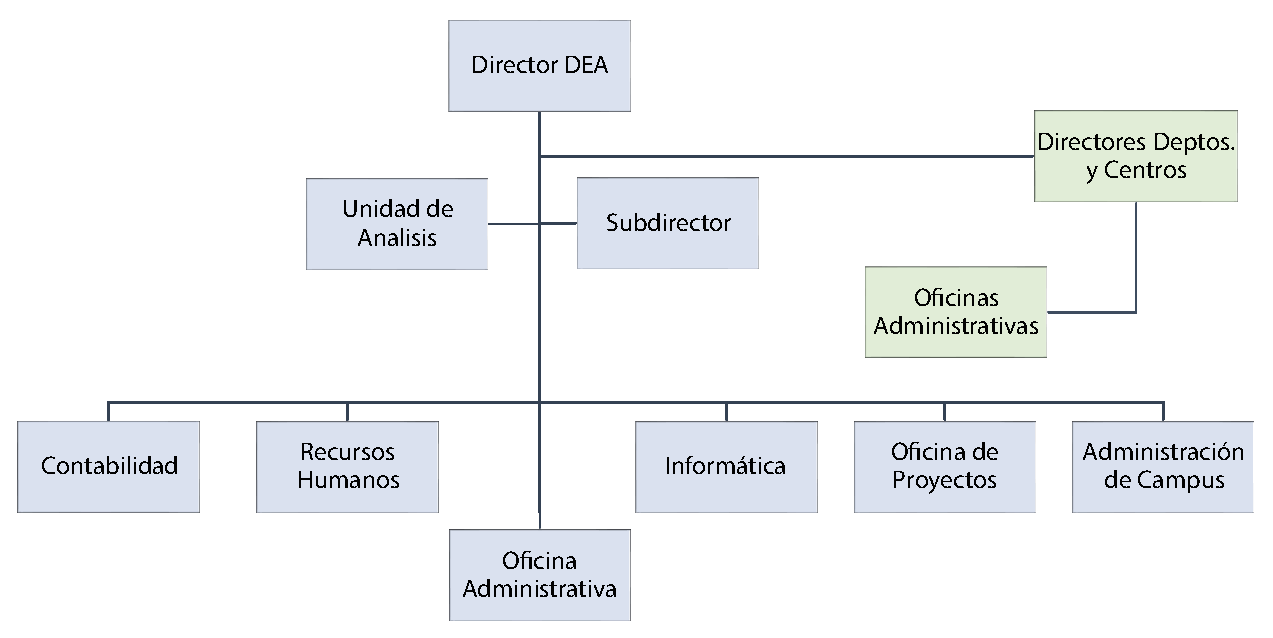
\includegraphics[width=\columnwidth]{./organigramas/organigrama_dea_fcfm.eps}
\caption{Organigrama de la Dirección Económica y Administrativa de la FCFM}
\label{ograma_dea_fcfm}
\end{figure}

La \textbf{Dirección Académica y de Investigación} tiene como misión contribuir, incentivar y
apoyar el desarrollo académico y la labor de investigación científica, tecnológica y de I\&D
en y entre las unidades académicas. Su propósito es, además, fomentar las actividades
multidisciplinarias. Entre sus prioridades institucionales se cuentan:

\begin{itemize}
\item Reforzar y transparentar la sistematización de la información en el área de investigación y
desarrollo facilitando y potenciando enfoques multidisciplinarios.
\item Apoyar a asesorar en el desarrollo académico a los Departamentos.
\item Contribuir a mantener el liderazgo en ciencia y tecnología, enfatizando la investigación como
parte fundamental de la labor académica.
\end{itemize}

La \textbf{Escuela de Ingeniería y Ciencias} tiene a su cargo la administración central de los planes de
estudio de pregrado y la coordinación de la enseñanza que imparten los departamentos académicos
de la Facultad.

La \textbf{Escuela de Postgrado} está encargada de organizar, administrar y coordinar los 23
programas de Magíster, 12 programas de Doctorado y los Diplomas de Postítulo ofrecidos por
la Facultad.

Los \textbf{Departamentos} que conforman la FCFM corresponden a:

\begin{enumerate}
\item Astronomía
\item Ciencia de los Materiales
\item Ciencias de la Computación
\item Física
\item Geología
\item Ingeniería Civil
\item Ingeniería de Minas
\item Ingeniería Eléctrica
\item Ingeniería Matemática
\item Ingeniería Mecánica
\item Ingeniería Química y Biotecnología
\end{enumerate}

La FCFM actualmente cuenta con 11 centros de investigación, en los que están involucrados
% más del <.#porcentaje_JC_en_CI_FCFM#.>\% del cuerpo académico de jornada completa, 
30 post-doctorantes.
% y <.#doctorado_en_CI_FCFM#.> tesistas de doctorado. 
Cada uno es líder en su disciplina en el país y en ellos se realiza la mayor actividad
de vinculación con el sector productivo y la sociedad, con énfasis en la creación de conocimiento,
desarrollo y transferencia tecnológica. Estos son:

\begin{itemize}
\item Centro de Modelamiento Matemático (CMM)
\item Centro Avanzado de Tecnología para la Minería (AMTC)
\item Centro de Excelencia en Geotermia de Los Andes (CEGA)
\item Instituto Sistemas Complejos de Ingeniería (ISCI)
\item Centro de Investigaciones en Energía Solar (SERC-Chile)
\item Centro de Ciencia del Clima y la Resiliencia (CR2)
\item Centro de Astrofísica y Tecnologías Afines (CATA)
\item Instituto Milenio de Astrofísica (MAS)
\item Centro de Biotecnología y Bioingeniería
\item Centro de Energía (CE)
\item Instituto Milenio para la Investigación de las Imperfecciones de Mercado y Política Pública (MIPP)
\end{itemize}

\subsection{Contexto de la FCFM}

\subsubsection{Oferta de títulos y grados de la FCFM}

La FCFM cuenta con una amplia oferta de título y grados. En pregrado, se ofrecen 10 carreras
profesionales que corresponden a Ingeniería Civil, Ingeniería Civil de Minas, Ingeniería Civil
en Biotecnología, Ingeniería Civil en Computación, Ingeniería Civil Eléctrica, Ingeniería Civil
Industrial, Ingeniería Civil Matemática, Ingeniería Civil Mecánica, Ingeniería Civil Química y
Geología; y 3 Licenciaturas en Astronomía, Física y Geofísica.

Además, cuenta con 23 programas de magíster en Astronomía, Computación, Física,
Geofísica, Geología, Ingeniería Eléctrica, Ingeniería Geotécnica, Ingeniería Química, Ingeniería
Sísmica, Ingeniería Mecánica, Metalurgia Extractiva, Recursos y Medioambiente Hídrico,
Transporte, Economía Aplicada, Gestión de Operaciones, Gestión y Dirección de Empresas,
Gestión y Políticas Públicas, Gestión para la Globalización, Ingeniería de Negocios con
Tecnologías de la Información, Ingeniería en Redes de Comunicaciones, Meteorología y
Climatología, Minería, Tecnologías de la Información.

Por último, la FCFM ofrece 12 programas de doctorado correspondientes a Astronomía,
Computación, Física, Geología, Ciencia de los Materiales, Fluidodinámica, Ingeniería Química,
Modelación Matemática, Ingeniería de Minas, Ingeniería Eléctrica, Sistemas de Ingeniería.

\subsubsection{Infraestructura de la FCFM} \label{infra_fcfm}

Campus Beauchef El Campus Beauchef de la Universidad de Chile alberga los edificios,
laboratorios, aulas, infraestructura deportiva y áreas verdes de la FCFM. Ubicado en la comuna
de Santiago, sus dependencias comprenden dos manzanas, encuadradas entre las calles Blanco
Encalada, Plaza Ercilla, Tupper y Club Hípico, separadas entre sí por la calle Beauchef, donde se
encuentra su entrada principal en Beauchef 850. El mapa del Campus Beauchef se muestra en la
Figura \ref{map_fcfm}.

\begin{figure}[ht!]
\centering
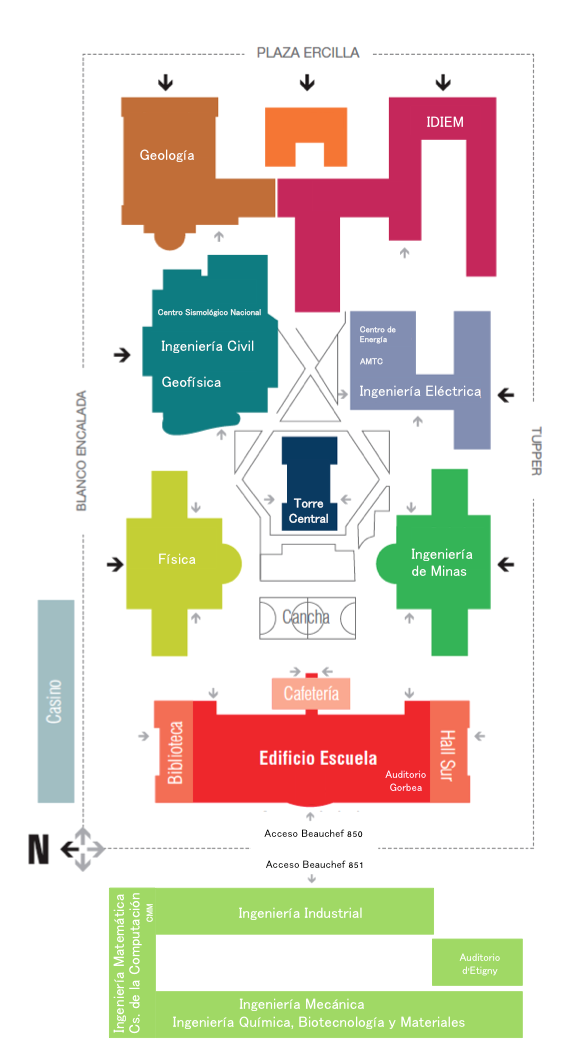
\includegraphics[width=0.94\columnwidth]{./pictures/mapa_fcfm.jpg}
\caption{Mapa Campus Beauchef}
\label{map_fcfm}
\end{figure}

El Campus Beauchef cuenta con 24 edificios, que suman 80.000 m$^2$ de superficie construida,
sobre un terreno de 36.000 m$^2$ donde se albergan más de 85 laboratorios con fines docentes y de
investigación.

La FCFM posee numerosos jardines que incluyen decenas de valiosas especies nativas y
foráneas, las cuales constituyen un interesante jardín botánico que adorna y da vida al Campus
Beauchef.

Los alumnos cuentan con una amplia sala con computadores centralizada, a la que se suman las
salas de computación disponibles en los Departamentos de Computación, Química y Biotecnología,
Mecánica, Civil, Eléctrica, Matemática, Geofísica, Geología y Astronomía.
Además, la Facultad cuenta con redes de comunicación de alta velocidad: fibra óptica y WiFi,
a disposición de todos los estudiantes, con acceso libre a Internet.

La FCFM posee más de 70 salas de clases, auditorios implementados con sofisticados equipos
para video conferencia, además de salas multimedia, y cómodas salas de estudio. En marzo de
2014 se instalaron modernas pizarras de acero porcelanizado, que es el material más moderno y
efectivo que existe en la actualidad para este tipo de trabajos, en 13 salas de Beauchef 850 y 8 salas
de Beauchef 851. Éstas fueron traídas desde EE.UU. y buscan darle más versatilidad a la enseñanza
en la Facultad.
La FCFM cuenta con un Sistema de Bibliotecas formado por la Biblioteca Central y
7 Bibliotecas Departamentales (Astronomía, Civil, Física, Geofísica, Geología, Industrias y
Matemáticas), con las más modernas tecnologías que permiten el acceso local y remoto a las
colecciones. Los otros Departamentos (Eléctrica, Mecánica, Química y Biotecnología, Minas)
decidieron tener un manejo centralizado de los volúmenes a través de la biblioteca central. El
sistema cuenta con un acervo bibliográfico de más de 185.000 volúmenes de libros, y acceso en
línea a: más de 52.000 revistas electrónicas y 150 bases de datos bibliográficas multidisciplinarias
y especializadas (con acceso a más de 2,2 millones de publicaciones en permanente actualización).
Para la realización de actividades deportivas la FCFM cuenta con múltiples espacios, que
corresponden a:

\begin{itemize}
\item Multicancha: Se encuentra al aire libre en el patio principal del campus Beauchef. En ella se
practica baby fútbol, voleibol y otros deportes en equipo.
\item Gimnasio, hubicado en Beauchef 851, está completamente
equipado con piscina, canchas de baloncesto, voleibol, tennis, racquetball y 
salas para actividades de musculación, preparación física, gimnasia aeróbica y taichí,
entre otras. 
\item Gimnasio Polideportivo Domeyko: Se emplaza en Almirante Latorre 730 y es un amplio
espacio que cuenta con equipamiento deportivo de primer nivel. Allí se practican deportes
como básquetbol, voleibol, tenis de mesa, gimnasia artística, judo, kárate y taekwondo, entre
otros.
\end{itemize}

Además, la Facultad tiene convenios para utilizar las instalaciones del Club de Tenis Santiago,
el Estadio Macul, el Estadio de Fútbol del Banco del Estado, la Piscina de la Universidad de Chile,
y otras dependencias deportivas de nuestra institución como el Refugio Cordillerano de Farellones.
El campus es complementado por instalaciones que lo rodean como el casino, ubicado en Blanco
Encalada 2085, y el Centro de Estudiantes de Ingeniería, en Tupper 2140.
La Facultad, además, cuenta con dependencias fuera del campus Beauchef, incluyendo el
Departamento de Ingeniería Industrial, ubicado en Avda. República 701; los laboratorios de
Ingeniería Mecánica, en Blanco Encalada 2743; y el Departamento de Astronomía, en el cerro
Calán, comuna de Las Condes, a los pies de la cordillera de Los Andes. Actualmente se encuentran
plenamente operativas las instalaciones del campus Beauchef 851.

Beauchef 851 es la más extensa ampliación en infraestructura del campus de la
FCFM desde su inauguración, hace más de un siglo. Este conjunto de edificaciones, emplazado
en la manzana poniente del campus, aumentó en un 50\% la infraestructura actual, y marca un hito
arquitectónico entre los espacios destinados a educación superior en Chile (ver Figura \ref{b851}). La
edificación cuenta con cerca de 50.000 m$^2$ construidos, distribuidos en siete pisos sobre superficie
y seis subterráneos. Allí se ubican salas de clases, laboratorios, oficinas, auditorios, espacios
deportivos y de recreación, y estacionamientos.

\begin{figure}[ht!]
\centering
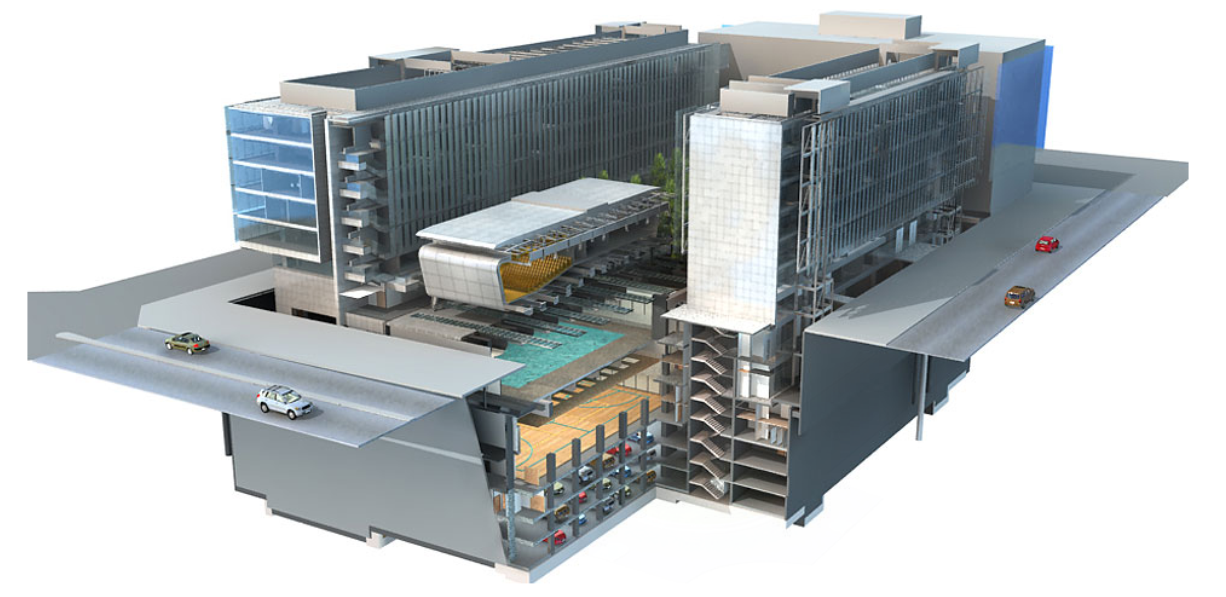
\includegraphics[width=\columnwidth]{./pictures/beauchef851.png}
\caption{Modelo tridimensional de Beauchef 851}
\label{b851}
\end{figure}

Uno de los sellos distintivos de Beauchef 851 es la eficiencia energética incorporada en su
diseño, construcción y operación, lo que permitirá certificarlo bajo los exigentes estándares LEED
ante el Consejo de Edificios Verdes de Estados Unidos (USGBC).

\subsubsection{Planta Docente de la FCFM}

La FCFM cuenta con 225 académicos de jornada completa (septiembre 2014) dedicados a la
investigación y/o innovación tecnológica para Chile y el mundo. También cuenta con más de
200 profesores con jornada parcial en contacto permanente con la industria.

En cuanto a los académicos de jornada completa, el 90\% de éstos posee el título de doctor
en el área donde hace clases e investigación y muchas veces incluyen a estudiantes dentro de sus
investigaciones, lo que aporta enormemente a su formación.
Entre el total de académicos – tanto jornada completa como parcial - casi el 70\% posee algún
tipo de postgrado. Además, la FCFM cuenta con más de 70 investigadores de postdoctorado. Éstos
y otros números se pueden ver en la Tabla \ref{jor_vs_grados}.

% Tabla 1.1
\begin{table}[ht!]
\centering
\caption{Número de docentes según jornada de contrato y grado académico.}
\label{jor_vs_grados}
\begin{tabular}{llllll}
\hline
Profesor         & \shortstack{Licenciados \\ o Titulados} 	& Con Magíster & Con Doctorado & Total & Con Postgrado \\ \hline \hline
Jornada Completa & 15	& 6 & 204 & 225 & 93,3\%          \\ \hline
Media Jornada    & 1 & 0 & 1 & 2 & 50\%          \\ \hline
Por Hora         & 123 & 39 & 61 & 223 & 44,8\%          \\ \hline
\textbf{Total}   & 139 & 45 & 266 & 450 & 69,1\%          \\ \hline
\end{tabular}
\end{table}

Los docentes del Plan Común, en gran parte, están adscritos a Departamentos de la FCFM,
principalmente a los Departamentos de Ingeniería Matemática, Física, Ingeniería Industrial,
Ciencias de la Computación y Ciencias de los Materiales. En el año 2013, de los 99 docentes
del Plan Común, 82 tenían grado de Doctor, 5 Magíster y 12 titulados y licenciados. De ese total
de docentes, 77 estaban a jornada completa y 22 eran contratados por hora.
Los académicos e investigadores de la FCFM publicaron 2.257 artículos científicos en revistas
ISI durante el año 2016. 
% El <.#porcentaje_con_factor_impacto_Q1#.>\% de las publicaciones ISI originadas en la Facultad tienen un factor de impacto Q1.

Desde el punto de vista de la jerarquización académica, la planta docente de la Facultad se
encuentra compuesta como se muestra en la Tabla \ref{jer_vs_grado}.

% Tabla 1.2
\begin{table}[hb!]
\centering
\caption{Número de docentes según jerarquía y grado académico.}
\label{jer_vs_grado}
\begin{tabular}{llllll}
\hline
Profesor        & \shortstack{Licenciados \\ o Titulados} & Con Magíster & Con Doctorado & Total & Con Postgrado \\ \hline \hline
Prof. Titular   & 17    & 4    & 70    & 91    & 81,3\%          \\ \hline
Prof. Asociado  & 20    & 4    & 77    & 101    & 80,2\%          \\ \hline
Prof. Asistente & 10    & 5    & 91    & 106    & 90,6\%          \\ \hline
Prof. Adjunto   & 40    & 12    & 17    & 69    & 42\%          \\ \hline
Inst. Adjunto   & 42    & 19    & 6    & 67    & 37,3\%          \\ \hline
Instructor      & 6    & 1    & 4    & 11    & 45,5\%          \\ \hline
Ayudante        & 4    & 0    & 0    & 4    & 0\%           \\ \hline
No Evaluado     & 0    & 0    & 1    & 1    & 100\%         \\ \hline
\textbf{Total}  & 139 & 45 & 266 & 450 & 69,1\%          \\ \hline
\end{tabular}
\end{table}

Otro factor importante en la formación de ingenieros y científicos es la presencia tanto de
académicos jóvenes como aquellos con más experiencia. Por esto, en la FCFM se han contratado
a cada vez más académicos jóvenes y esto puede demostrarse con la información entregada en la
Figura \ref{etario}, donde cerca del 46,8\% de los académicos son menores de 50 años.

\begin{figure}[ht!]
\centering
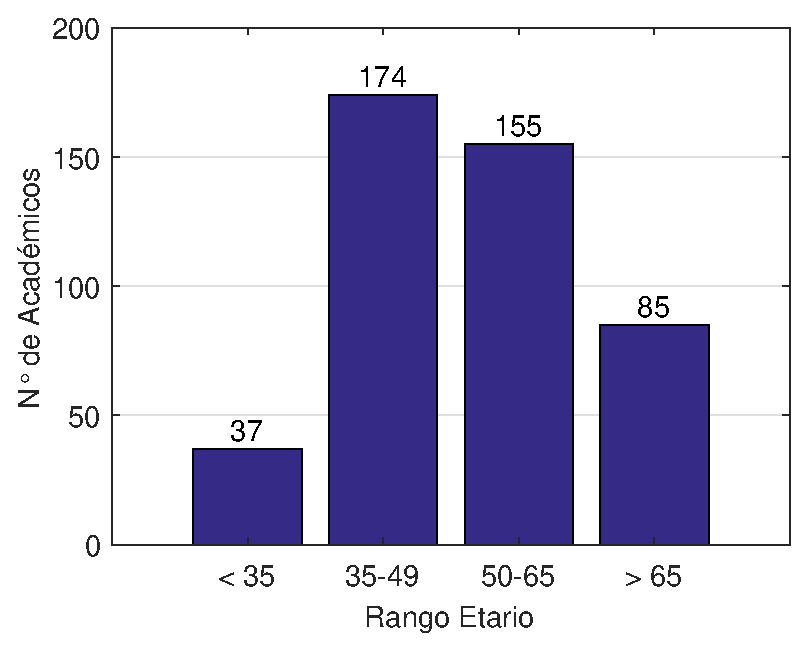
\includegraphics[width=0.65\columnwidth]{./pictures/etario.eps}
\caption{Rango etario de académicos de la FCFM.}
\label{etario}
\end{figure}

\subsubsection{Perfil de los estudiantes de la FCFM}\label{prefil_fcfm}

A la Escuela de Ingeniería y Ciencias ingresaron 695 alumnos (ingreso regular) el año 2014. Así,
los jóvenes que se unen a esta Facultad se incorporan a una institución viva, que se actualiza y
renueva constantemente, difundiendo conocimientos y estableciendo estándares para la docencia
y la investigación en ingeniería y ciencias afines, formación que es reconocida a nivel nacional e
internacional.

%La principal vía de admisión es a través de la Prueba de Selección Universitaria (PSU) según
%las ponderaciones indicadas en la Tabla \ref{psu}.

%\begin{table}[ht]
%\centering
%\caption{Ponderación puntajes de ingreso a la FCFM.}
%\label{psu}
%\begin{tabular}{lll}
%\hline
%                                  & 2003-2011 & 2012-presente \\ \hline \hline
%Prueba de Matemáticas             & 50\%      & 45\%          \\ \hline
%Prueba de Lenguaje y Comunicación & 10\%      & 10\%          \\ \hline
%Prueba de Ciencias                & 20\%      & 15\%          \\ \hline
%Notas de Enseñanza Media          & 20\%      & 10\%          \\ \hline
%Ranking de Egreso                 & 0\%       & 20\%          \\ \hline
%\end{tabular}
%\end{table}

%Inicialmente se ingresa a un programa de Plan Común. Este es un período de estudios que dura
%4 semestres y que entrega una sólida base en física y matemática, necesaria para desenvolverse en
%el mundo tecnológico de hoy. La ventaja de esta modalidad, utilizada en las universidades más
%prestigiosas, es que posterga la elección de la carrera a los recién egresados de Enseñanza Media,
%hasta una etapa en que los intereses de los alumnos están más definidos.

%Procedencia de los alumnos La Universidad de Chile se caracteriza por la diversidad de sus
%alumnos, y en la FCFM no es la excepción. La Tabla \ref{ingreso_fcfm} indica la procedencia de los alumnos que
%ingresan a Plan Común según tipo de establecimiento, donde se puede apreciar que más de la mitad
%de los alumnos provienen de establecimientos municipales o subvencionados. 

%\begin{table}[!ht]
%\centering
%\caption{Ingreso a la FCFM por tipo de establecimiento.}
%\label{ingreso_fcfm}
%\begin{tabular}{llll}
%\hline
%Año                                                                                & 2011 & 2012 & 2013 \\ \hline \hline
%\begin{tabular}[c]{@{}l@{}}N$\circ$ de alumnos de primer año que provienen \\ de establecimientos municipales\end{tabular}          & 189  & 154  & %152  \\ \hline
%\begin{tabular}[c]{@{}l@{}}N$\circ$ de alumnos de primer año que provienen \\ de establecimientos subvencionados\end{tabular}       & 182  & 200  & %220  \\ \hline
%\begin{tabular}[c]{@{}l@{}}N$\circ$ de alumnos de primer año que provienen \\ de establecimientos particulares pagados\end{tabular} & 357  & 332  & %312  \\ \hline
%Sin información                                                                    & 0    & 2    & 5    \\ \hline
%\textbf{Total}                                                                     & 728  & 688  & 689  \\ \hline
%\end{tabular}
%\end{table}


Los estudiantes que
ingresan a la FCFM son parte del 3\% superior de rendimiento en la PSU. El puntaje de cierre de
ingreso se encuentra por sobre los 712.3 puntos, mientras que los máximos puntajes ingresados llegan
hasta los 840.1 puntos. La Figura \ref{puntajes_psu} muestran los puntajes PSU máximo, mínimo y promedio de
ingreso al Plan Común en los últimos años.

\begin{figure}[ht!]
\centering
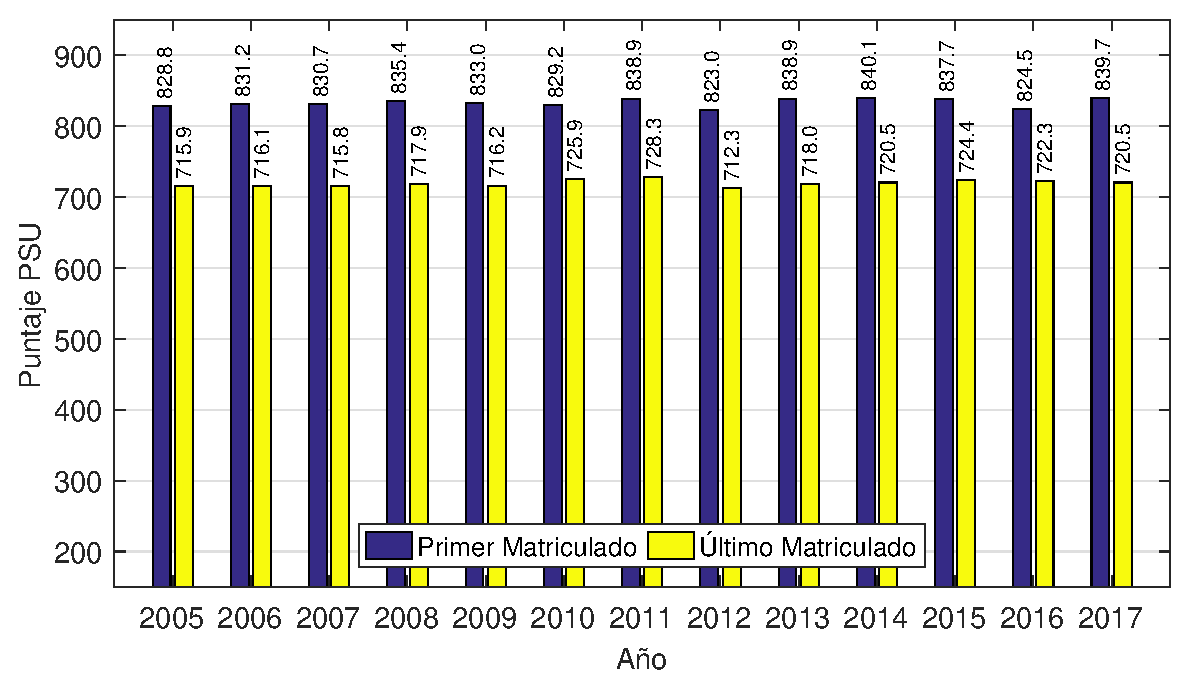
\includegraphics[width=\columnwidth]{./pictures/puntajes_psu.eps}
\caption{Puntajes de Ingreso a la FCFM.}
\label{puntajes_psu}
\end{figure}

%Como se observa en la Tabla \ref{ingreso_regiones}, a la FCFM ingresan alumnos provenientes de todas las
%regiones del país, confiando en que recibirán la mejor formación en ingeniería y ciencias. Si bien
%la mayor parte reside en la Región Metropolitana, alrededor de un <.#ingreso_otras_regiones_FCFM#.>\% de los alumnos son de otras
%regiones, siendo la <@regiones_mas_representadas@> región las más representadas.

%\begin{table}[!ht]
%\centering
%\caption{Procedencia de alumnos por regiones (2012).}
%\label{ingreso_regiones}
%\begin{tabular}{lccccccc}
%\hline
%Región                   & I   & II  & III  & IV  & V    & VI   & VII  \\ \hline \hline
%Ingreso               & <.#in_reg(1)#.>\% & <.#in_reg(2)#.>\% & <.#in_reg(3)#.>\%    & <.#in_reg(4)#.>\% & <.#in_reg(5)#.>\%  & <.#in_reg(6)#.>\%  %& <.#in_reg(7)#.>\%  \\[0.3cm] \hline
%\multicolumn{1}{r}{VIII} & IX  & X   & XI   & XII & RM   & XIV  & XV   \\ \hline \hline
%\multicolumn{1}{r}{<.#in_reg(8)#.>\%}  & <.#in_reg(9)#.>\% & <.#in_reg(10)#.>\% & <.#in_reg(11)#.>\% & <.#in_reg(12)#.>\%   & <.#in_reg(13)#.>\% & %<.#in_reg(14)#.>\% & <.#in_reg(15)#.>\% \\ \hline
%\end{tabular}
%\end{table}


%Desde hace algunos años, el porcentaje de mujeres en la Facultad se ha mantenido estable
%alrededor del 20\% (ver Tabla \ref{infreso_genero}), cifra muy superior a Facultades de Ingeniería de otras
%Universidades, en las que el número de mujeres es muy reducido. Desde 2014, se comenzó a
%implementar el Programa de Ingreso Prioritario de Equidad de Género, que considera el aumento
%de 40 cupos especiales para mujeres que queden en lista de espera, y así mejorar su participación
%en la comunidad de la FCFM.

%\begin{table}[ht]
%\centering
%\caption{Procedencia de alumnos por género.}
%\label{infreso_genero}
%\begin{tabular}{lccccccccc}
%\hline
%Año     & <#ano_in(1)#> & <#ano_in(2)#> & <#ano_in(3)#> & <#ano_in(4)#> & <#ano_in(5)#> & <#ano_in(6)#> & <#ano_in(7)#> & <#ano_in(8)#> & %<#ano_in(9)#>   \\ \hline \hline
%Mujeres & <.#in_muj(1)#.>\% & <.#in_muj(2)#.>\% & <.#in_muj(3)#.>\% & <.#in_muj(4)#.>\% & <.#in_muj(5)#.>\% & <.#in_muj(6)#.>\% & <.#in_muj(7)#.>\% %& <.#in_muj(8)#.>\% & <.#in_muj(9)#.>\% \\ \hline
%Hombres & <.#in_hom(1)#.>\% & <.#in_hom(2)#.>\% & <.#in_hom(3)#.>\% & <.#in_hom(4)#.>\% & <.#in_hom(5)#.>\% & <.#in_hom(6)#.>\% & <.#in_hom(7)#.>\% %& <.#in_hom(8)#.>\% & <.#in_hom(9)#.>\% \\ \hline
%\end{tabular}
%\end{table}

\subsection{Descripción de la unidad y su proceso de enseñanza-aprendizaje}

La FCFM comenzó hace más de diez años, de forma pionera, una revisión profunda de sus
currículos de carreras y programas, de los contenidos de sus asignaturas y de sus métodos docentes.
Este rediseño se ha enmarcado dentro del modelo desarrollado por la Iniciativa CDIO (Concibe,
Diseña, Implementa y Opera), que agrupa alrededor de un centenar de escuelas de ingeniería en el
mundo, que trabajan en conjunto para mejorar su enseñanza. La Escuela de Ingeniería y Ciencias
de la FCFM es responsable de liderar la región latinoamericana de CDIO.

La experiencia adquirida en la aplicación del nuevo plan de estudios, iniciado en 2007, ha
demostrado la importancia de que los cambios curriculares vayan acompañados de cambios en las
metodologías de enseñanza-aprendizaje, que coloquen al estudiante al centro del proceso educativo.
Esto coincide con la disponibilidad creciente de tecnología, tanto para el profesor como para los
alumnos. A menudo, esta tecnología ha venido a reforzar los métodos expositivos tradicionales, que
mantienen al alumno en un rol pasivo (por ejemplo, a través el uso de PowerPoint), pero esa misma
tecnología tiene también la potencialidad de generar múltiples oportunidades de Aprendizaje
Activo. Bajo este concepto, que es uno de los estándares de CDIO, se agrupan todos los métodos
docentes que involucran activamente al alumno en la sala de clases y en la construcción de su
aprendizaje.

%A partir de noviembre 2013, el Área de Desarrollo Docente (ADD) de la FCFM se encuentra
%ejecutando el proyecto MECESUP UCH1305 denominado ``Fortalecimiento de la capacidad de
%innovación en la enseñanza y aprendizaje en la FCFM''. Este proyecto tiene por objetivo general
%instalar e impulsar la utilización de métodos de aprendizaje activo de los estudiantes de pregrado de
%la FCFM, fortaleciendo para ello la capacidad de la unidad de mejoramiento docente para apoyar
%a los profesores en la adopción y uso de métodos docentes innovadores, centrados en el alumno,
%que incorporen las prácticas actuales más adecuadas a nuestras carreras y estudiantes; además se
%considera la habilitación de espacios apropiados para la implementación de estos métodos. Cabe
%destacar que con la reforma curricular de los años 2007-2009 se definió un nuevo perfil de egreso,
%y se construyeron programas de cursos dentro de un modelo de docencia para introducir un sistema
%curricular basado en competencias. Se incluyeron estrategias didácticas para generar aprendizajes
%activos en los estudiantes. El ADD de la FCFM ha apoyado el nuevo diseño curricular y su
%implementación, incluyendo capacitación de los docentes en las nuevas metodologías.

\subsubsection{Habilidades de comunicación oral y escrita en español}

En el caso del idioma español, desde el año 2010 se hace un diagnóstico en primer año del Plan
Común llamado Prueba de Competencias Discursivas de Comprensión y de Escritura (CODICE).
CODICE tiene como propósitos aportar información a las unidades académicas sobre el desempeño
de los estudiantes de primer año en Lectura y Escritura, y obtener datos para hacer estudios
de validez predictiva sobre este instrumento, como herramienta complementaria a la Prueba de
Selección Universitaria.

El proyecto MECESUP UCH1302 tiene como propósito desarrollar ``Estrategias para mejorar
las habilidades de lecto-escritura de los estudiantes de 1er y 2do año de la Universidad de Chile,
a partir de los resultados de la prueba CODICE''. Este programa apunta a la nivelación de las
competencias de entrada que sean deficitarias.

Diversos diagnósticos, en base tanto a opiniones de académicos, egresados y empleadores,
como a través de la prueba CODICE, coinciden en que nuestros estudiantes requieren desarrollar
de mejor manera sus habilidades de comunicación. Para esto, se formó un equipo, con el apoyo de
un proyecto FADOP (Fondo de Apoyo a la Docencia de Pregrado) de la Universidad de Chile, que
formuló una estrategia con un enfoque similar al de la ética: combinando el apoyo de expertos
con el trabajo de los profesores en algunas asignaturas. El plan trazado está en proceso de
implementación.

\subsubsection{Habilidades de comunicación oral y escrita en inglés}

Las competencias comunicativas en el idioma inglés forman parte fundamental del perfil de egreso
de los estudiantes de la carrera de Ingeniería Civil Eléctrica (ICE) y de la FCFM en general.
Atendiendo a esta necesidad, la Facultad creó el Área de Inglés, cuyo propósito es que los
estudiantes logren desenvolverse comunicacionalmente de manera efectiva en forma oral y escrita
en esta lengua, en temáticas generales de la vida diaria. El Programa de Inglés rediseñado el
2007 consta de cinco niveles, dicta 225 horas totales de docencia directa del programa, con un
enfoque primordialmente comunicativo, en los cuales los cursos no exceden los 20 estudiantes.
Adicionalmente, desde el año 2012, se ha integrado al Programa de Inglés el sistema Duolingo\footnote{\url{https://es.duolingo.com/}}
que consiste en una plataforma web, gratuita, en donde el estudiante realiza ejercicios diversos
y va avanzando cuando cumple los requisitos de cada etapa. Para aquellos estudiantes con
dificultades estructurales para aprender idiomas se implementó un programa tutorial, que cuenta
con un proceso de postulación, previa recomendación de sus profesores. La metodología utilizada
consiste en conversación de pares, preguntas y respuestas entre compañero y profesor, juegos de
roles, conversaciones grupales y actividades lúdicas, además de las prácticas personales con el
sistema Duolingo.

Para aprobar el programa de inglés los estudiantes deben obtener un puntaje igual o superior
a 75\% en el test de Michigan, que es equivalente a 513 puntos del Test de TOEFL, lo cual los deja
capacitados para:

\begin{itemize}
\item Inferir información a partir de textos auditivos extensos y variados
\item Debatir y argumentar sobre diferentes tópicos con mayor fluidez, claridad y precisión
\item Hacer presentaciones de tópicos más profundos de la vida diaria como son los sentimientos,
música, hábitos de sueño, etc.
\item Analizar textos de mayor complejidad sobre tópicos abstractos
\item Reconocer términos y expresiones más coloquiales dentro de un texto
\end{itemize}

\section{Departamento de Ingeniería Eléctrica}

El Departamento de Ingeniería Civil Eléctrica (DIE) es el encargado de coordinar y administrar los
programas de Magíster y Doctorado de Ingeniería Eléctrica, así como la carrera de Ingeniería Civil
Eléctrica en el ciclo posterior al Plan Común, hasta la graduación o titulación.

En diciembre de 1945 se decide en el Consejo de la FCFM que todos los ingenieros titulados en la
FCFM llevarán el título genérico de Ingeniero Civil en el caso de todas las carreras de ingeniería
impartidas por la Facultad. Siguiendo los importantes desarrollos que estaba experimentando
el país con la creación de CORFO y ENDESA, en 1946 se establecieron cuatro carreras que
compartían un Plan Común de tres años de duración. Entre ellas estuvo la Ingeniería Mecánica
Electricista.

En junio de 1949 la Comisión de Docencia recomendó cambiar el nombre de las carreras
Ingeniería Mecánica Industrial e Ingeniería Mecánica Electricista por los de Ingeniería Civil
Industrial e Ingeniería Civil Electricista, respectivamente. Este cambio fue solicitado al Consejo
Universitario en abril de 1950.

En enero de 1957 fue inaugurado, por la FCFM de la Universidad de Chile en conjunto con la
Empresa Nacional de Electricidad Sociedad Anónima ENDESA, el Instituto de Investigaciones y
Ensayos Eléctricos (IIEE). En 1965 se convirtió en el Departamento de Electricidad y en 1981 se
constituyó como Departamento de Ingeniería Eléctrica.

\begin{figure}[ht!]
\centering
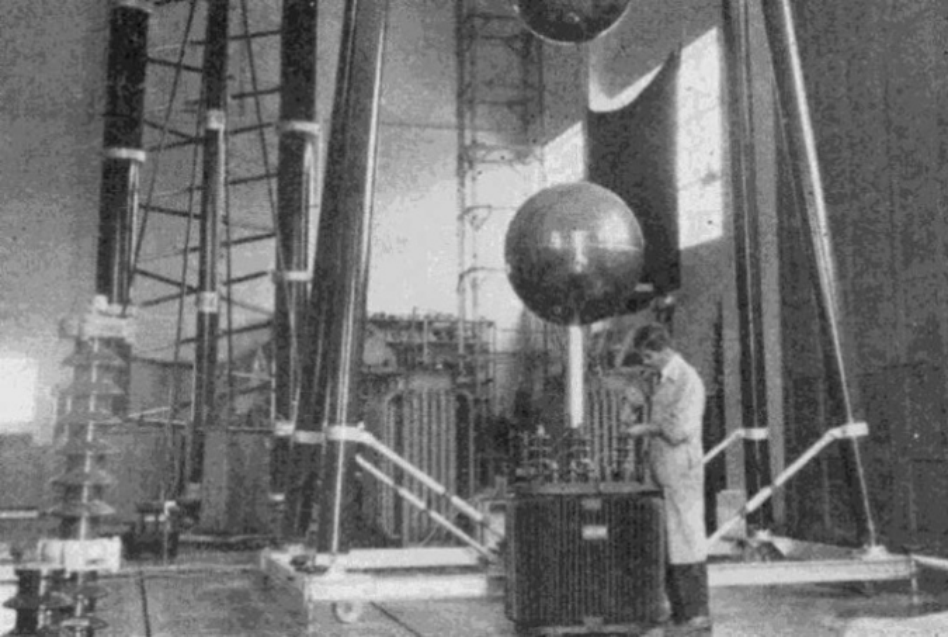
\includegraphics[width=\columnwidth]{./pictures/historia_DIE.png}
\caption{Laboratorio del Instituto de Investigaciones y Ensayos Eléctricos.}
\label{hist_die}
\end{figure}

El IIEE fue constituido por el Laboratorio de Alta Tensión, el Laboratorio de Electrotecnia y
el Laboratorio de Electrónica y Telecomunicaciones. Luego de tres años, se incluyó el Laboratorio
de Computadores y Control Automático.

En el período 1968 – 1969 en la Facultad se llevaron a cabo cambios y creaciones de gran
importancia, aprovechando un período que, en parte, fue motivado por la influencia global que
tuvieron los eventos estudiantiles ocurridos en Francia durante ese período. En este período se
realizó en la Facultad una substancial reforma docente. Se revisaron los planes de estudio y los
programas de los cursos y se instauró un sistema semestral, en vez del sistema anual.

En 1969, con apoyo de la Organización de Estados Americanos OEA, se creó el primer
programa de Magíster en Ingeniería Eléctrica. El Departamento había sido declarado Centro de
Excelencia por la OEA. Por una parte, esto permitió contratar profesores de Estados Unidos y
Europa; por otra, varios alumnos extranjeros pudieron seguir el programa y obtener el grado
de magíster. En el año 1985, en concordancia con una evolución y expansión de las áreas del
departamento, se crea el actual programa de Magíster en Ciencias de la Ingeniería, Mención
Eléctrica.

En 2005, se creó el programa de Doctorado en Ingeniería Eléctrica del que se han graduado
32 doctores y que actualmente cuenta con 53 alumnos.

El año 2006 se inició un profundo proceso de Reforma Curricular de las distintas
especialidades de las carreras de Ingeniería Civil, implementándose a partir de los ingresados el año
2007 al Plan Común de Ingeniería y a partir de 2009 para la especialidad de Ingeniería Eléctrica.
El Decreto Universitario N$^\circ$~0025028 [\ref{dec25028}] de 10 de octubre de 2008 de la Universidad de Chile,
estableció el nuevo plan de estudios para la licenciatura en Ciencias de la Ingeniería, mención
Eléctrica, y para la carrera de Ingeniería Civil Eléctrica. Este mismo decreto establece el cambio
de nombre de la carrera de Ingeniería Civil Electricista, pasando a llamarse Ingeniería Civil
Eléctrica.

Para la Reforma Curricular del 2007-2009 se realizó la elaboración de programas de cursos de
la carrera, proponiendo nuevas metodologías docentes, unificando criterios de evaluación y malla
de requisitos, e incluyendo en estos nuevos programas de curso las competencias profesionales y
genéricas de la carrera. Se implementaron estrategias metodológicas de aprendizaje y enseñanza
en varios cursos de la carrera.

El decreto Universitario N$^\circ$~0027663 [\ref{dec27663}] de 5 de noviembre de 2008 incorporó la variable de
género en grados académicos y títulos profesionales de la Universidad de Chile.

En el año 2007 la carrera Ingeniería Civil Electricista se sometió por primera vez a un proceso
de acreditación ante la Comisión Nacional de Acreditación (CNAP), donde fue acreditada por el
máximo de 7 años. En el último proceso del año 2015, la carrera de Ingeniería Civil Eléctrica fue
acreditada nuevamente por el máximo de 7 años, que culminan el 23 de enero de 2022. Por su parte,
el Programa de Magíster en Ciencias de la Ingeniería Mención Eléctrica, se encuentra acreditado
por un período de 6 años que finalizan el 21 de abril de 2016. A su vez el programa de Doctorado
se encuentra acreditado por un período de 8 años hasta el 09 de noviembre de 2019.

Entre los logros históricos del DIE se encuentran:
\begin{itemize}
\item En 1957 contribuyó con la planificación de la electrificación del país.
\item En 1962 instaló, operó y administró el primer computador digital en la Universidad de Chile.
\item En 1969, con apoyo de la OEA, creó el primer programa de Magíster en Ingeniería Eléctrica.
\item En 1973 diseñó y construyó el primer transistor bipolar en Chile.
\item En 1974 organizó el primer Congreso Chileno en Ingeniería Eléctrica y creó la Asociación Chilena de Control Automático (ACCA).
\item En 1976 diseñó y construyó el primer circuito integrado en el país.
\item En el año 1985 creó el actual programa de Magíster en Ciencias de la Ingeniería, Mención Eléctrica.
\item En 2005 creó el actual programa de Doctorado en Ingeniería Eléctrica.
\item En 2007 diseñó y construyó el primer automóvil de energía solar en Chile.
\item En 2007 DIE firma acuerdo con Associated Universities Inc. (AUI) que opera y administra el Atacama Large Millimeter Array (ALMA).
\item En 2009 se creó el programa de Magíster en Ingeniería de Redes de Comunicaciones. 
\item En marzo de 2009 se crea el Centro Avanzado de Tecnología para la Minería (AMTC).
\item En junio de 2009 nace el Centro de Energía (CE).
\item En 2010 diseñó, construyó y puso en marcha la primera micro-red inteligente con Energías Renovables No Convencionales (ERNC).
\item En 2014 se crea ECODIE, unidad de Educación Continua del DIE.
\item En 2015 se crea la primera plataforma solar del país instalada en Atacama.
\item En 2017 se lanza el primer satélite chileno al espacio.
\item En 2017 programa de doble doctorado en Ingeniería Eléctrica U. de Chile y U. de Nottingham tiene su primer graduado.

\end{itemize}

\subsection{Contexto del DIE}

\subsubsection{Infraestructura del DIE}

El DIE cuenta con un edificio de 8 pisos de propiedad institucional (6 sobre suelo y 2
subterráneos), donde se encuentran 6 salas de clases, oficinas administrativas y de los académicos
del departamento, salas de reuniones, laboratorios docentes y de investigación, un taller metalmecánico y una moderna sala de computadores.

\begin{figure}[ht!]
\centering
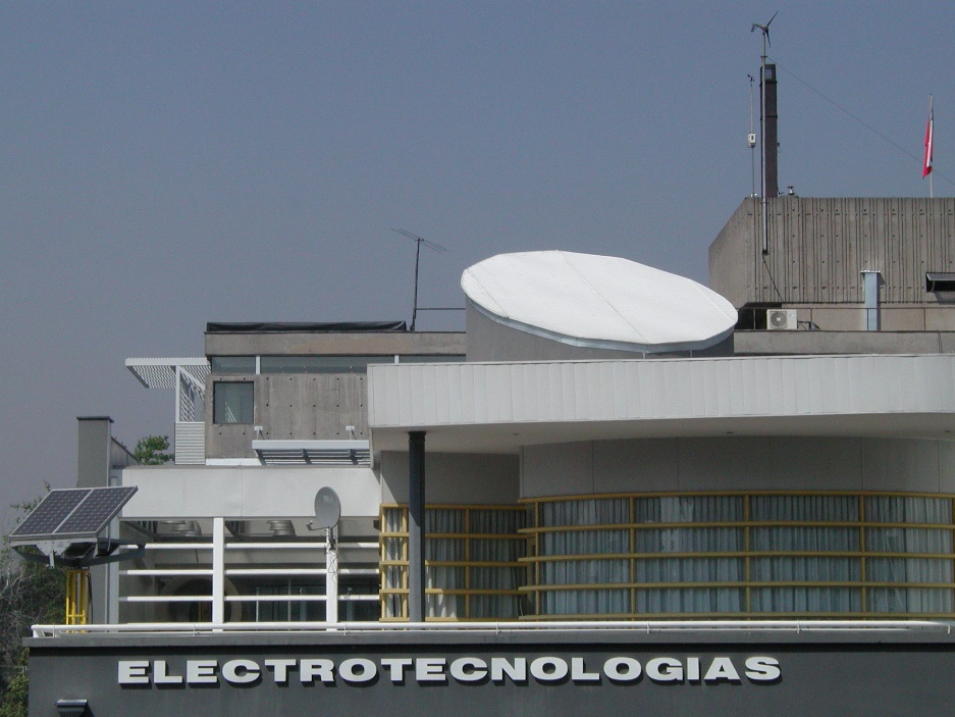
\includegraphics[width=\columnwidth]{./pictures/electrotecnologias.png}
\caption{Edificio de Electrotecnologías.}
\label{edif_ET}
\end{figure}

El DIE posee una infraestructura para labores docentes y experimentales de excelencia, lo
que permite un adecuado desarrollo de sus actividades de formación e investigación. Cuenta
hoy día con la infraestructura más importante del país en la especialidad con alrededor de
7.000 m$^2$. Esto incluye el edificio de Electrotecnologías, remodelado el año 2003, donde
se dispone de 8 laboratorios docentes de pregrado de ICE. Además, existen 15 laboratorios
de investigación en el departamento. Académicos y estudiantes trabajan conjuntamente en la
resolución de problemas complejos utilizando tecnologías de punta. Estas actividades cuentan
con financiamiento gubernamental de CONICYT, CORFO y MILENIO, así como también de
organizaciones internacionales y de aportes empresariales. El funcionamiento de los laboratorios
de investigación, así como la compra de equipamiento menor y mayor, se financia adecuadamente
con los proyectos de investigación dirigidos por los académicos del DIE.

La Tabla \ref{labs_die} muestra que a través de fondos concursables e inversiones de Facultad y DIE
se han creado 6 laboratorios nuevos a partir del año 2008, con una inversión total de
\$1.692.500.000. Cabe destacar que el Laboratorio de Ondas Milimétricas y Sub-milimétricas
es parte de una colaboración entre el DIE y el DAS, y se encuentra físicamente en este último.
Además el laboratorio es liderado por el Dr. Patricio Mena (académico del DIE) en conjunto con el
Dr. Leonardo Bronfman (académico del DAS).

\begin{table}[t!]
\centering
\caption{Inversión en Laboratorios Nuevos DIE desde el año 2007.}
\label{labs_die}
\begin{tabular}{lll}
\hline
& Año & Fuentes  \\ \hline \hline %& Inversión {[}CLP{]}
Laboratorio de Fotónica & 2008 & FCFM; CONICYT \\ %& 178.000.000 \\
\begin{tabular}[c]{@{}l@{}}Laboratorio de Ondas \\ Milimétricas y \\ Submilimétricas\end{tabular} & 2008 & \begin{tabular}[c]{@{}l@{}}Centro Basal de \\ Astrofísica y \\ Tecnologías Afines; \\ Fondos Concursables\end{tabular} \\ % & 870.000.000 \\
\begin{tabular}[c]{@{}l@{}}Laboratorio de \\ Exploración Espacial \\ y Planetaria (LEEP)\end{tabular} & 2010 & SUCHAI \\ % & 4.000.000 \\
\begin{tabular}[c]{@{}l@{}}Laboratorio de \\ Electrónica de Potencia, \\ Accionamientos y \\ Generación Distribuida\end{tabular} & 2011 & \begin{tabular}[c]{@{}l@{}}FCFM; DIE; \\ FONDECYT; \\ FONDEQUIP\end{tabular} \\ % & 600.000.000 \\
Optical \& Wireless Laboratory & 2011 & \begin{tabular}[c]{@{}l@{}}FCFM; DIE; \\ VID; FONDECYT\end{tabular} \\ % & 19.000.000 \\
Laboratorio de Acumuladores & 2012 & FCFM; DIE; CIL \\ \hline % & 21.500.000 \\ \hline
% & & \multicolumn{1}{r}{\textbf{TOTAL}} \\ \hline %& <.#laboratorioDIE.total_inversion#.> \\ \hline
\end{tabular}
\end{table}

\subsubsection{Planta Docente del DIE}

%La Tabla \ref{horas_jornada} presenta el número de académicos de jornada completa y parcial para los últimos <.#total_de_anos#.>
%años. Al <#planta_docente_ano(3)#> el cuerpo docente de Ingeniería Civil Eléctrica se compuso de <.#docentes_JC_DIE(3)#.> de académicos de
%jornada completa con doctorado, y <.#docentes_hora_DIE(3)#.> académicos de jornada parcial. Dentro del cuerpo académico,
%además de doctores en ingeniería eléctrica, se encuentran expertos de las industrias involucradas
%en la carrera como lo son: telecomunicaciones, energía, automática, etc.

%\begin{table}[ht]
%\centering
%\caption{Número y horas docentes de la carrera, según jornada de contrato.}
%\label{horas_jornada}
%\begin{tabular}{llll}
%\hline
%Año                                 		& <#planta_docente_ano(1)#> & <#planta_docente_ano(2)#> & <#planta_docente_ano(3)#> 
%N$^\circ$~docentes jornada completa        	& <.#docentes_JC_DIE(1)#.>  & <.#docentes_JC_DIE(2)#.>  & <.#docentes_JC_DIE(3)#.>  \\
%Horas docentes\footnote{Horas efectivas de clases a la semana} jornada completa    		& <.#horas_docentes_JC_DIE(1)#.>  & <.#horas_docentes_JC_DIE(2)#.>  & <.#horas_docentes_JC_DIE(3)#.>  \\
%											&   &   &   \\
%N$^\circ$~docentes contratados por hora    	& <.#docentes_hora_DIE(1)#.>  & <.#docentes_hora_DIE(2)#.>  & <.#docentes_hora_DIE(3)#.>  \\
%Horas docentes contratados por hora 		& <.#horas_docentes_hora_DIE(1)#.>  & <.#horas_docentes_hora_DIE(2)#.>  & <.#horas_docentes_hora_DIE(3)#.>  \\
%											&   &   &   \\ \hline
%Total docentes                      		& <.#docentes_DIE_total(1)#.>  & <.#docentes_DIE_total(2)#.>  & <.#docentes_DIE_total(3)#.>  \\
%Total horas                         		& <.#horas_docentes_DIE_total(1)#.>  & <.#horas_docentes_DIE_total(2)#.>  & <.#horas_docentes_DIE_total(3)#.>  \\ \hline
%\end{tabular}
%\end{table}

En la Tabla \ref{docentes_grados} pueden observarse las estadísticas de los académicos según grado académico
en el DIE. Todos los profesores de jornada completa del DIE poseen el grado de doctor, mientras
que entre los profesores de jornada parcial hay 3 doctores y 6 magísteres.

\begin{table}[ht]
\centering
\caption{Número de docentes según grado académico.}
\label{docentes_grados}
\begin{tabular}{llll}
\hline
Año                        			& 2017 \\ \hline \hline %2011 & 2012 & 2013 \\ \hline \hline
N$^\circ$~Doctores (PhD)        	& 28 \\ %21  & 22  & 24  \\
N$^\circ$~Magíster              	& 6 \\ %6  & 6  & 6  \\
N$^\circ$~Licenciados o titulados 	& 15 \\ %37  & 34  & 32  \\ \hline
\textbf{Total}             			& 49 \\ %64  & 62  & 62  \\ \hline
\end{tabular}
\end{table}

\subsubsection{Perfil de los estudiantes del DIE}

El DIE recibe a sus alumnos provenientes del Plan Común de la FCFM, cuyo perfil se
encuentra detallado en la Sección \ref{prefil_fcfm} ``Perfil de los estudiantes de la FCFM''.

Una de las principales fortalezas de los alumnos que ingresan a estudiar la carrera de Ingeniería
Civil Eléctrica, es su alto nivel académico. La Figura \ref{puntajes_psu_ice} muestra los promedios ponderados PSU
para estudiantes del Plan Común y de Ingeniería Civil Eléctrica. Se observa que los puntajes
obtenidos por los estudiantes de ICE, se encuentran por encima del promedio del Plan Común de
la Facultad.

\begin{figure}[ht]
\centering
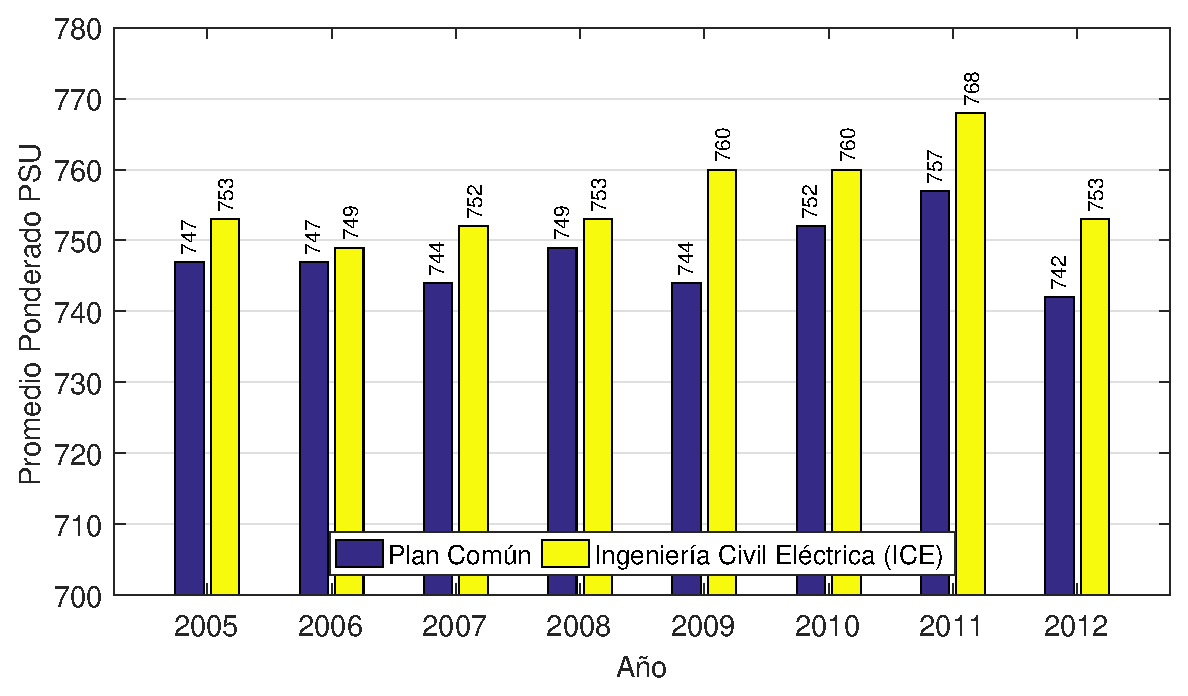
\includegraphics[width=\columnwidth]{./pictures/puntajes_psu_ice.eps}
\caption{Puntajes promedio PSU para estudiantes del Plan Común y del ICE.}
\label{puntajes_psu_ice}
\end{figure}

%En cuanto a género, se ve una disminución en el porcentaje de mujeres que ingresa a la carrera,
%con respecto al Plan Común. En este último, las mujeres representan cerca del 20\% del total de los
%estudiantes, mientras que en ICE es apenas cercano al 7\%. La Tabla \ref{matricula_genero} muestra el número de
%estudiantes de ICE por género entre los años 2011 y 2013.

%\begin{table}[ht]
%\centering
%\caption{Matrícula por género a ICE.}
%\label{matricula_genero}
%\begin{tabular}{llll}
%\hline
%Año                     & <#anos_estadisticas_genero_DIE(1)#> & <#anos_estadisticas_genero_DIE(2)#> & <#anos_estadisticas_genero_DIE(3)#> \\ %\hline \hline
%Matrícula total hombres & <.#matricula_hombres_ice(1)#.>  & <.#matricula_hombres_ice(2)#.>  & <.#matricula_hombres_ice(3)#.>  \\
%Matrícula total mujeres & <.#matricula_mujeres_ice(1)#.>  & <.#matricula_mujeres_ice(2)#.>  & <.#matricula_mujeres_ice(3)#.>  \\ \hline
%\textbf{Total}          & <.#matricula_total_ice(1)#.>  & <.#matricula_total_ice(2)#.>  & <.#matricula_total_ice(3)#.>  \\ \hline
%\end{tabular}
%\end{table}

\subsection{Descripción de la unidad académica}

El esquema docente en la FCFM, basado en un Plan Común inicial, está diseñado para lograr
que nuestros estudiantes alcancen un muy buen nivel base en Matemáticas y Física, permitiendo
un máximo aprovechamiento de las temáticas tratadas con posterioridad. La gran fortaleza del
Plan Común consiste en entregar herramientas para una adecuada adaptación de los educandos
a los veloces cambios en el conocimiento. Por otro lado, los estudiantes deciden finalmente
su especialidad, de manera informada y fundada, al cabo de 4 semestres de permanencia en la
Facultad. La FCFM ofrece 10 diferentes carreras profesionales y 3 licenciaturas, a las que acceden
nuestros estudiantes posteriormente a su aprobación del Plan Común, entre ellas Ingeniería Civil
Eléctrica (ICE). El año 2007 comenzó la más profunda reforma curricular de la carrera de Ingeniería
Civil Eléctrica de los últimos 40 años. Para esto se definió un nuevo perfil de egreso basado en
competencias que se desarrollan a lo largo de la carrera y que fueron agrupadas en competencias
profesionales (técnicas) y competencias genéricas, las cuales se encuentran publicadas en la página
web del DIE\footnote{\url{http://www.die.cl}}. El perfil de egreso antiguo se basaba en los contenidos de las materias para declarar
las habilidades requeridas por el profesional que egresaba. Para el nuevo plan de estudio, la
definición de perfil de egreso se centra en las habilidades para aprender y utilizar los contenidos,
lo cual se define como las competencias. En particular se utilizó la metodología CDIO. Las
competencias del nuevo perfil se diseñaron tomando en cuenta los adelantos en la disciplina, los
propósitos y misión de la institución, y se validó con empresarios externos.

\section{Magíster en Ingeniería de Redes de Comunicaciones}

\subsection{Breve historia del Programa}

Desde sus orígenes, la Universidad de Chile ha hecho contribuciones de primera importancia a
la formación del pensamiento crítico y al desarrollo de la nación. En docencia de postgrado
se revela una tradición que comienza en el año 1947 con la creación del primer doctorado en
Filosofía de la Facultad de Filosofía y Educación, y que se extiende hasta hoy con el sistema
de postgrado y postítulo más grande y complejo del país, compuesto por 36 programas de
doctorado, 118 programas de magíster, 75 programas de título profesional especialista y 27 cursos
de especialización de postítulo. El Departamento de Ingeniería Eléctrica es un fiel exponente de
esto, en donde destaca hoy en día el Doctorado en el área tecnológica con más años de acreditación
en la Universidad de Chile (8 años)5. Una fortaleza importante radica en la reglamentación existente
que cubre políticas institucionales de desarrollo del postgrado, estándares, calidad exigida a los
profesores y estudiantes, exigencias de investigación.

% En el año 1985, en concordancia con una evolución y expansión de las áreas del departamento,
% se crea el actual programa de Magíster en Ciencias de la Ingeniería, Mención Eléctrica [A.4]. No
% obstante, nuestro departamento tiene una larga historia en programas de Magíster, donde destaca
% el Magíster de Ingeniería Eléctrica que data de 1969. El Programa ha sido acreditado dos veces
% por la CONAP (actual CNA). El primer proceso fue el 2005 donde fue acreditado por un periodo
% de 4 años [A.5], siendo re-acreditado el 2010 por 6 años [A.6]. Esto lo posiciona dentro de los
% programas con mayor años de acreditación dentro de su área en la Universidad de Chile. El actual
% proceso corresponde a una segunda re-acreditación que apunta a un tramo de evaluación mayor, en
% relación a las mejoras realizadas desde la última acreditación.

En el 2010, el programa de Magíster en Ingeniería de Redes de Comunicaciones nace para atender la urgente necesidad que durante la primera década de nuestro siglo aquejaba a la industria de las telecomunicaciones en Chile, a saber, la falta de profesionales con especialización en tecnologías IP que tuvieran una formación neutra y un conocimiento agnóstico a lo que ofrecían los proveedores de tecnología.

Fue en una continuidad natural del postítulo en Internetworking, también de nuestra universidad, que formó cerca de 200 profesionales realizaron el desarrollo de sus habilidades prácticas con los laboratorios del Departamento de Ingeniería Electrica de la Facultad de Ciencias Físicas y Matemáticas. La proyección de los ex-alumnos de este postítulo requerían un complemento que les permitiera ampliar sus conocimientos de Internetworking, fundamentalmente en Routing, Switching IP y Telefonía tanto circuital como de paquetes IP, y poder ejercer su profesión en los operadores de telecomunicaciones que por esa fecha se perfilaban como convergentes tanto en tecnologías (circuitos y paquetes) como en servicios (telefonía y datos).

Es en ese contexto en que el programa se dicta por primera vez en el año 2010, con el incondicional impulso del entonces director del DIE, el profesor Nicolás Beltrán Maturana. Los tres primeros graduados del programa, dictado en un formato de magíster profesional al estilo de MBA de las telecomunicaciones con elementos de Informática, incorporando las tecnologías inalámbricas de punta en esos días, hacen sus recuerdos: “El ingreso y estadía en el programa MIRC se debe en gran parte al director del departamento de ese momento, el profesor Sr. Nicolás Beltrán, quién siempre me ayudo en el aspecto académico y administrativo“, dice Alberto Castro. Por su parte, Jorge Sandoval, al igual que Castro, un profesional de primera línea en nuestra industria, comenta: “La formación que recibí en el MIRC me abrió muchas puertas y el mercado reconoció mi condición de magíster aplicado a las necesidades de nuestra industria y con gran potencial de actualización, especialmente en las tecnologías y los servicios inalámbricos“. El tercero de la primera generación de graduados, Minflen Torres, también destacó por su orientación a las tecnologías inalámbricas dada su sólida formación en el MIRC, desarrollando una excelente carreta profesional en Entel, operador en el que trabaja hasta la actualidad.
La llegada del profesor Claudio Estévez en el año 2013 como coordinador al programa, le dio impulso a un programa diversificado que incluyó tópicos de Cloud Computing, IoT, Big Data Analytics, Evolución de 4G a 5G, Smart Cities, Regulación y Economía en las Telecomunicaciones, entre otros  temas de punta tanto tecnológica como de negocios, imprimiendo un enfoque fuertemente orientado a las necesidades de la industria de telecomunicaciones de estos días en que los operadores convergentes son una realidad que coexiste con los operadores Over The Top y los operadores virtuales.

El cuerpo académico, tanto en el claustro como en el equipo extendido de profesionales que trabajan en la industria, ha evolucionado desde Beltrán hasta Estévez para mantener actualizada la oferta de materias, siempre considerando las necesidades del país, la formación y en el perfeccionamiento de profesionales que destaquen por su visión sistémica y sus sólidos conocimientos tanto teóricos como prácticos.


\subsection{Proyecto académico de la unidad}

Este Programa otorga una formación con énfasis en la ingeniería avanzada y tecnologías
modernas de las redes de comunicación, que permitan a los graduados contribuir al desarrollo de sus países y satisfacer las
necesidades de la sociedad. Ofrece una formación profunda para
aquellas personas que desean orientar sus estudios hacia actividades de innovación tecnológica y docencia superior.

Lo(a)s ingeniero(a)s que ingresan pueden profundizar sus estudios en áreas como Smart Cities, Internet de las Cosas, Cloud Computing, 
técnicas de modulación, protocols de acceso, protocolos de transporte, enrutamiento, comunicación vehicular, eficiencia energética
en sistemas de comunicación, modelamiento de redes, calidad de servicio y experiencia en redes móviles, comunicación inalámbrica avanzada, 
seguridad de redes y muchos otros tópicos más. El cuerpo académico cubre una amplia diversidad de tópicos, esto para poder cumplir 
los objetivos del programa.
